\section{Evaluación de la adaptación}
\label{sec:marco-evaluacion}
La evaluación externa examina las respuestas ante consultas distintas de las utilizadas para entrenar y permite estudiar si los cambios se mantienen fuera de la señal de recompensa. Su interpretación requiere identificar el benchmark, las condiciones de generación y el evaluador, además de definir cómo se agregan los criterios.

\subsection{HealthBench y evaluación por conversación}
\label{sec:marco-healthbench}
HealthBench es un benchmark desarrollado por OpenAI para evaluar respuestas médicas abiertas mediante criterios específicos de cada conversación, elaborados por profesionales médicos~\cite{arora2025healthbench}. Además de su versión general, el benchmark incluye las variantes HealthBench Hard y HealthBench Consensus, por lo que es necesario identificar de cuál procede cada evaluación.

El procedimiento conserva la conversación y su identificador, genera una respuesta al último mensaje del usuario y evalúa cada criterio a partir de esa respuesta y del contexto disponible. Las respuestas se guardan antes de calificarlas, mientras que las decisiones del juez y sus explicaciones se almacenan en archivos separados, lo que permite revisar una decisión individual o recalcular las métricas sin volver a generar el texto. Como muestra la figura \ref{fig:protocolo-evaluacion}, la rúbrica de HealthBench se proporciona únicamente al juez, de modo que el modelo evaluado responde sin acceder a esos criterios. Estas rúbricas pertenecen a la evaluación externa y deben distinguirse de las utilizadas como recompensa durante el entrenamiento.

\begin{figure}[htbp]
\centering
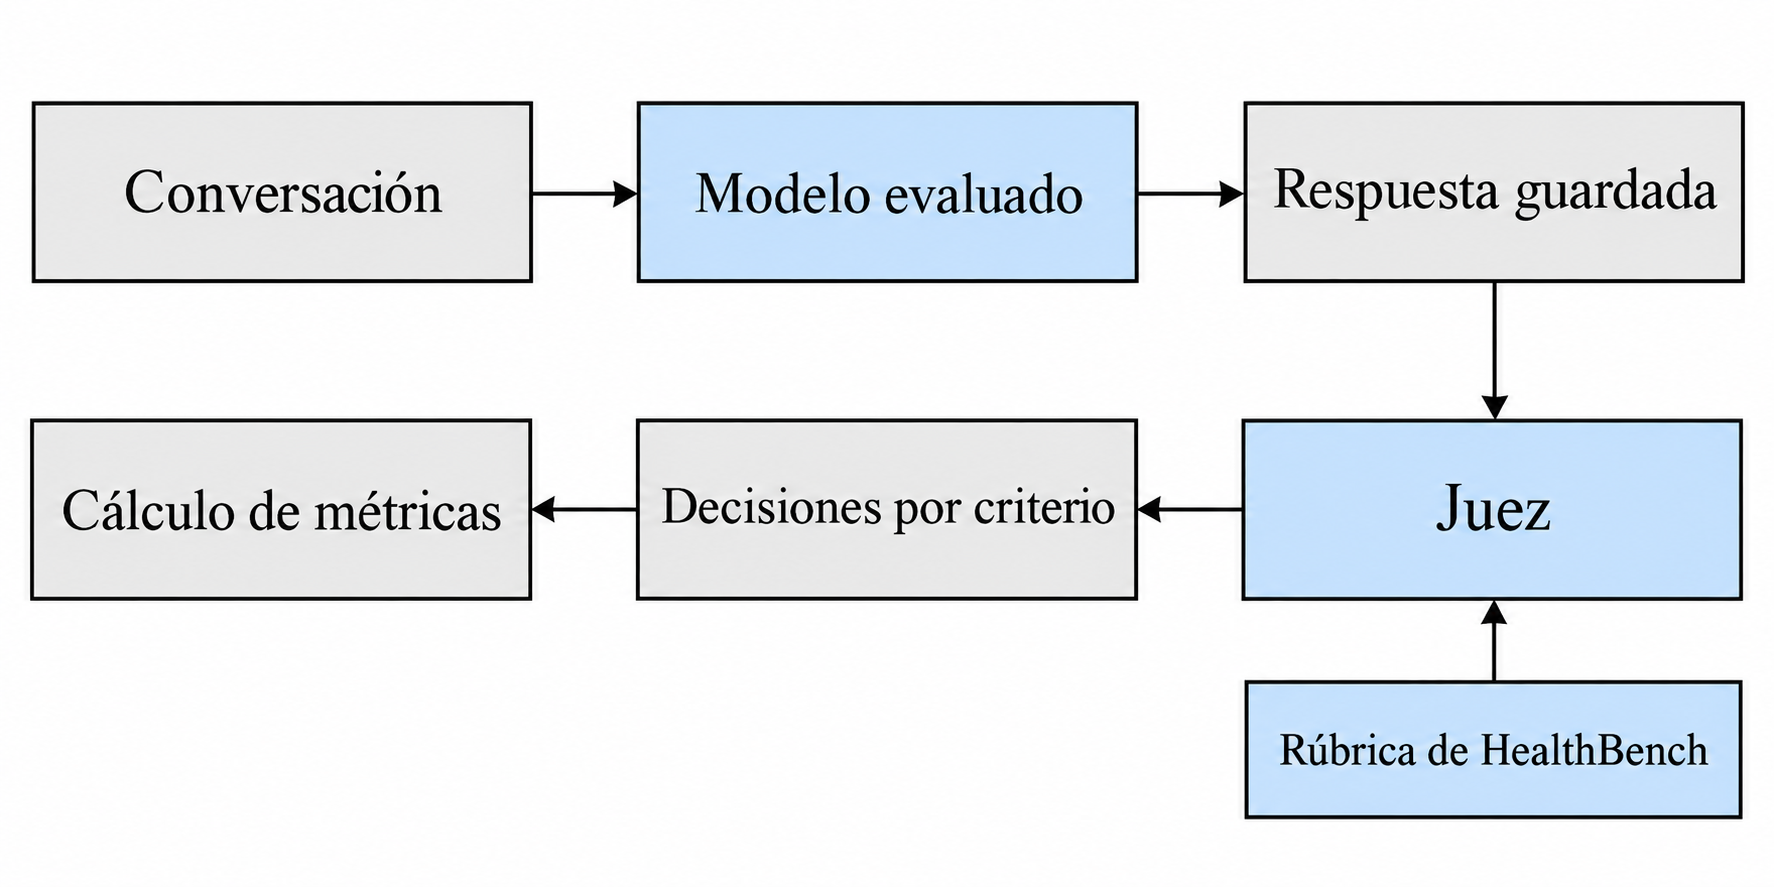
\includegraphics[width=0.95\textwidth]{Figuras/02-marco-teorico/06-evaluacion/evaluacion-protocolo.png}
\caption{Evaluación de respuestas mediante las rúbricas de HealthBench y un modelo juez.}
\label{fig:protocolo-evaluacion}
\end{figure}

Las condiciones concretas de la muestra, la generación y el juez del proyecto se describen en la sección~\ref{sec:protocolo-experimental}.

\subsection{Métricas y comparación de modelos}
\label{sec:evaluacion-metricas}
El puntaje principal combina los criterios cumplidos y sus pesos. Para el caso $i$, sea $p_{ij}$ el peso del criterio $j$ y $m_{ij}\in\{0,1\}$ la decisión de cumplimiento del juez. Si existen puntos positivos disponibles, el valor crudo del caso es
\begin{equation}
s_i=\frac{\sum_{j=1}^{M_i}p_{ij}m_{ij}}
{\sum_{j=1}^{M_i}\max(p_{ij},0)},
\label{eq:healthbench-caso}
\end{equation}
donde $M_i$ es la cantidad de criterios del caso. El numerador incorpora los puntos positivos obtenidos y las penalizaciones activadas, mientras que el denominador representa los puntos positivos disponibles. Por lo tanto, cumplir un criterio de peso negativo resta puntos y puede producir un valor individual negativo.

Para $N$ casos evaluados, el resultado global expresado en porcentaje se calcula como
\begin{equation}
S=100\,\operatorname{clip}\!\left(\overline{s},0,1\right),
\qquad \overline{s}=\frac{1}{N}\sum_{i=1}^{N}s_i.
\label{eq:healthbench-global}
\end{equation}
El orden de estas operaciones sigue el apéndice D de HealthBench y la implementación de simple-evals~\cite{arora2025healthbench,openai2026healthbenchcode}. Primero se promedian los valores crudos y después se recorta el promedio al intervalo indicado, por lo que recortar cada caso antes de promediar corresponde a otro cálculo. En consecuencia, en la formulación de HealthBench un resultado agregado en el extremo inferior puede provenir del recorte de una media neta no positiva y no equivale a que la totalidad de las respuestas sea incorrecta. Por esta razón, el benchmark prevé documentar el comportamiento de las respuestas sin limitarse al puntaje agregado recortado, incorporando desgloses por componentes y el balance de penalizaciones.

El análisis también considera los cinco ejes asociados a los criterios de HealthBench~\cite{arora2025healthbench}, que permiten describir distintos aspectos de una respuesta:

\begingroup
\begin{itemize}
\item \textbf{Precisión:} evalúa la corrección de la información médica y de las recomendaciones, considerando si la respuesta incluye afirmaciones erróneas o presenta como ciertos datos que no están suficientemente respaldados.
\item \textbf{Completitud:} considera si la respuesta cubre la información necesaria para resolver la consulta, incluyendo explicaciones, recomendaciones y advertencias pertinentes, sin omitir aspectos relevantes para el paciente.
\item \textbf{Calidad de comunicación:} examina si la información se presenta de forma clara, comprensible y organizada, con un lenguaje adecuado al interlocutor y un tono que facilite entender las recomendaciones.
\item \textbf{Comprensión del contexto:} valora si la respuesta tiene en cuenta los antecedentes, los síntomas y las circunstancias descritas en la conversación, ajustando sus explicaciones y recomendaciones a la situación particular.
\item \textbf{Seguimiento de instrucciones:} comprueba si la respuesta respeta las solicitudes y restricciones aplicables, como el idioma, el formato o el alcance pedido, manteniendo la atención en lo que se consulta.
\end{itemize}
\endgroup

Para un eje $a$, se calcula el valor del caso utilizando únicamente sus criterios y se incluyen en la agregación los casos con puntos positivos disponibles para ese eje. Si $I_a$ reúne esos casos, el desglose se expresa como
\begin{equation}
s_i^{(a)}=\frac{\sum_{j\in a}p_{ij}m_{ij}}{\sum_{j\in a}\max(p_{ij},0)},
\qquad S^{(a)}=100\,\operatorname{clip}\!\left(
\frac{1}{|I_a|}\sum_{i\in I_a}s_i^{(a)},0,1\right).
\label{eq:healthbench-ejes}
\end{equation}
De este modo, la agregación respeta el peso y la normalización de cada caso, en lugar de promediar directamente porcentajes de criterios cumplidos. En este informe, los desgloses por eje se utilizan para describir el comportamiento de las respuestas bajo el juez local y se presentan separados del puntaje principal.

Como indicadores complementarios, se contabilizan los criterios positivos cumplidos y los criterios negativos activados, expresados como proporciones dentro de cada grupo. Estos conteos no incorporan los pesos, por lo que deben distinguirse de las contribuciones ponderadas al puntaje. Para estudiar ese balance, se separan por caso los términos positivos y negativos del numerador de la ecuación \ref{eq:healthbench-caso}, manteniendo el mismo denominador, y luego se promedian sus contribuciones. Así puede observarse si una mayor cobertura se acompaña de más penalizaciones, sin interpretar todos los criterios negativos como medidas exclusivas de daño clínico.

La comparación pareada utiliza los mismos identificadores para ambos modelos y conserva los valores crudos. Si $s_i^{\mathrm{GRPO}}$ y $s_i^{\mathrm{SFT}}$ son sus respectivos puntajes, se define
\begin{equation}
d_i=s_i^{\mathrm{GRPO}}-s_i^{\mathrm{SFT}},
\qquad \overline{\Delta}=\frac{100}{N}\sum_{i=1}^{N}d_i,
\label{eq:healthbench-pareado}
\end{equation}
con lo que pueden contarse los casos favorables a cada modelo y los empates, además de estimar la diferencia media en puntos porcentuales. El recorte puede ocultar diferencias cuando ambos promedios quedan por debajo de cero o por encima de uno, por lo que también se compara la media de los puntajes crudos. Por otra parte, la longitud de las respuestas, la cobertura de criterios y los errores de evaluación se registran como indicadores descriptivos, sin presentarlos como métricas oficiales adicionales ni como pruebas directas de calidad.

La incertidumbre se estima mediante remuestreo bootstrap de casos. La implementación consultada utiliza 1.000 remuestreos con reemplazo y devuelve la desviación estándar de los puntajes globales recortados, identificada como bootstrap\_std~\cite{openai2026healthbenchcode}. Cuando se informa además un intervalo percentil del 95\%, sus límites se obtienen de los percentiles 2,5 y 97,5 de la distribución remuestreada, por lo que la desviación estándar y el intervalo no constituyen la misma medida. En la comparación entre modelos se remuestrean los mismos casos para ambos y se recalcula la diferencia en cada repetición, conservando así el emparejamiento tanto para la media cruda como para los resultados globales.

El análisis de las métricas se complementa con la revisión de respuestas concretas, especialmente cuando una mayor cobertura se acompaña de más penalizaciones. Examinar esos casos permite distinguir qué información se añadió y qué errores detectó el juez, así como identificar decisiones que requieren revisión experta.%
